\section{Ordenación por inserción}
El algoritmo de ordenación por inserción es un algoritmo sencillo que funciona de la siguiente manera:
\begin{enumerate}
    \item \textbf{Selecciona} el segundo elemento de la lista,
    \item \textbf{verifica} si es menor que el primer elemento, si es así, lo intercambia con el primer elemento,
    \item \textbf{Selecciona} el tercer elemento de la lista,
    \item \textbf{verifica} si es menor que el segundo elemento, si es así, lo intercambia con el segundo elemento, y \textbf{verifica} si es menor que el primer elemento, si es así, lo intercambia con el primer elemento,
    \item y así sucesivamente hasta que el conjunto esté ordenado.
\end{enumerate}

\subsection{Recurso gráfico}
Para ilustrar el funcionamiento del algoritmo de ordenación por inserción, se ha desarrollado un recurso gráfico que permite visualizar el estado del conjunto en cada iteración. Supongamos que se tiene la lista:
\begin{equation*}
    [ \ 9,3,1,3,5,27 \ ]
\end{equation*}

\begin{figure}[H]
    \centering
    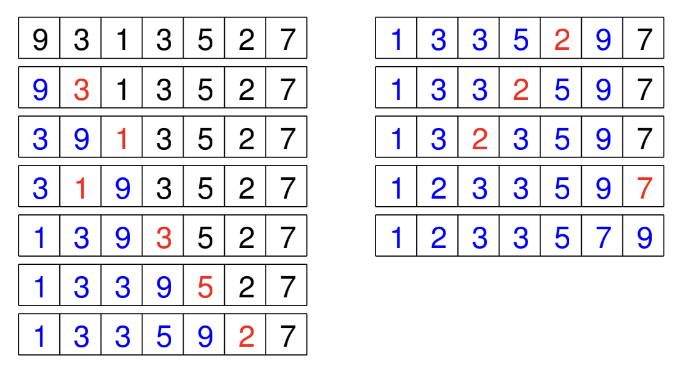
\includegraphics[scale=0.5]{./Images/oedei.png}
    \caption{Paso a paso de la ordenación por inserción.}
\end{figure}

\subsection{Código}

\begin{pascallike}
proc insertion_sort (in/out a: array[1..n] of T)
    for i:= 2 to n do
        insert(a,i)
    od
end proc
proc insert (in/out a: array[1..n] of T, in i: nat)
    var j: nat
    j:= i
    do j > 1 && a[j] < a[j - 1] -> 
        swap(a,j-1,j)
        j:= j-1
    od
end proc
\end{pascallike}

Para el algoritmo de ordenación por inserción, se ha desarrollado un procedimiento \texttt{insertion\_sort} que recibe un arreglo de tamaño $n$ y lo ordena. El procedimiento \texttt{insertion\_sort} utiliza un procedimiento auxiliar \texttt{insert}. El procedimiento \texttt{insert} recibe un arreglo y una posición, y mueve el elemento en la posición dada a la posición correcta. Se puede definir de una forma mas abreviada el algoritmo de ordenación por inserción, como se muestra a continuación:

\begin{pascallike}
proc insertion_sort (in/out a: array[1..n] of T)
    for i:= 2 to n do
        j:= i
        do j > 1 && a[j] < a[j - 1] -> 
            swap(a,j-1,j)
            j:= j-1
        od
    od
end proc
\end{pascallike}